\documentclass[12pt]{article}
\usepackage{graphicx}
\usepackage{graphicx}
\usepackage{float}
\usepackage[export]{adjustbox}
\usepackage{amsmath}
\usepackage{amssymb}
\usepackage{listings}
\usepackage{subcaption}
  
%
% Title.
\title{EE 324: Problem Sheet-2}

% Author
\author{Abhilaksh Kumar, 18D070035}

% begin the document.
\begin{document}

% make a title page.
\maketitle

\section{PROBLEM-1}
The entire code snippet :-
    \begin{figure}[H]
        \centering
        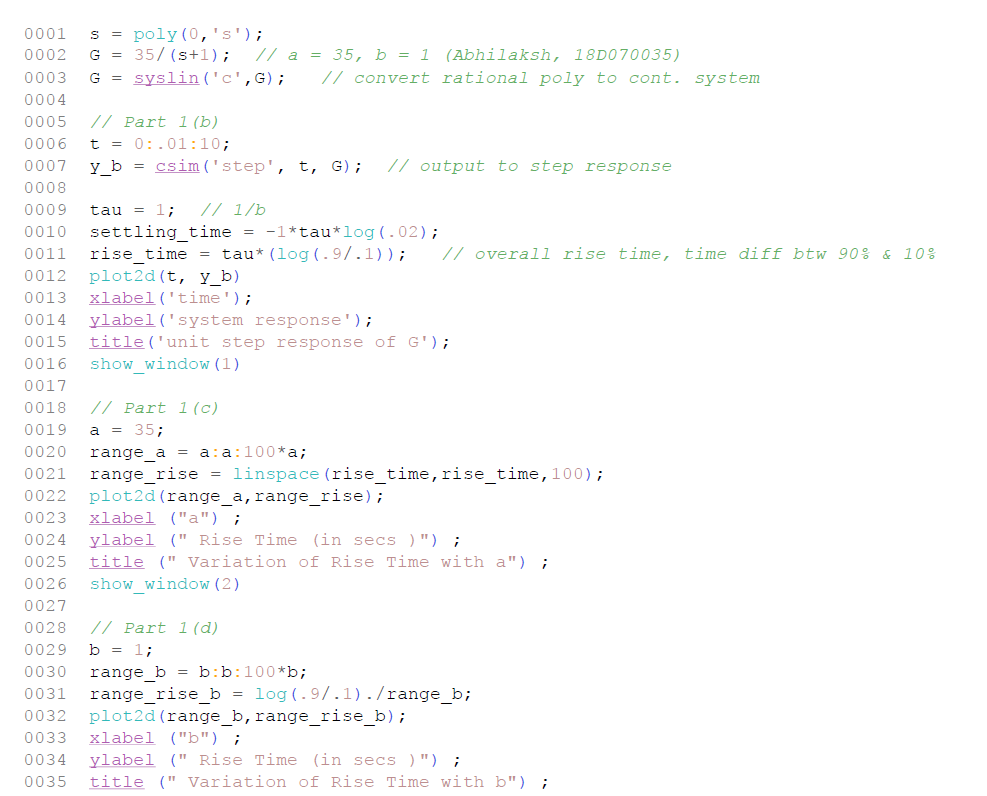
\includegraphics[scale=0.8]{q1_code.png}
    \end{figure}
    \vspace{-2mm}
\subsection*{Part a \& b}
\begin{itemize}
\item Name is Abhilaksh Kumar
\item Roll No is 18D070035
\end{itemize}

\begin{verbatim}
s = poly(0,'s');
G = 35/(s+1);  // a = 35, b = 1 (Abhilaksh, 18D070035)
G = syslin('c',G);   // convert rational poly to cont. system

// Part 1(b)
t = 0:.01:10;
y_b = csim('step', t, G);  // output to step response

tau = 1;  // 1/b
settling_time = -1*tau*log(.02);
rise_time = tau*(log(.9/.1));   // overall rise time, time diff btw 90% & 10%
plot2d(t, y_b)
xlabel('time');
ylabel('system response');
title('unit step response of G');
show_window(1)
\end{verbatim}
    \begin{figure}[H]
        \centering
        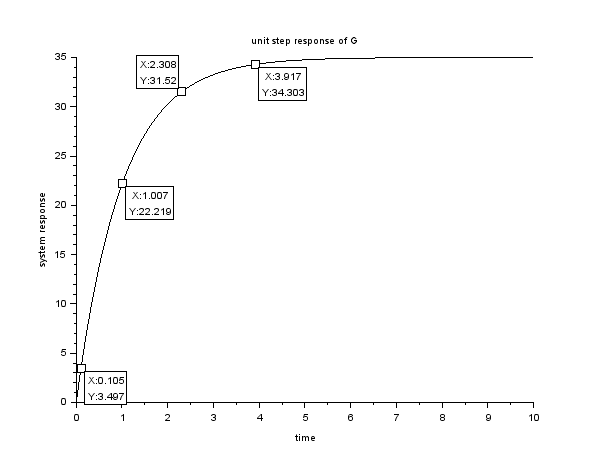
\includegraphics[scale=0.8]{q1_a.png}
        \caption{Step Response of G}
        \label{fig:my_label}
    \end{figure}
 
\subsection*{Part c}   
\begin{itemize}
\item Rise time between 90\% and 10\%
\item Steady state value is a/b 
\item Time constant = 1 unit
\item For settling time, we want time such that y = .98*a/b
\end{itemize}    
It remains constant with respect to variation in a
The code for that is:-
    \vspace{-2mm}
    \begin{verbatim}
a = 35;
range_a = a:a:100*a;
range_rise = linspace(rise_time,rise_time,100);
plot2d(range_a,range_rise);
xlabel ("a") ;
ylabel (" Rise Time (in secs )") ;
title (" Variation of Rise Time with a") ;
show_window(2)
    \end{verbatim}
    \vspace{-6mm}
    \begin{figure}[H]
        \centering
        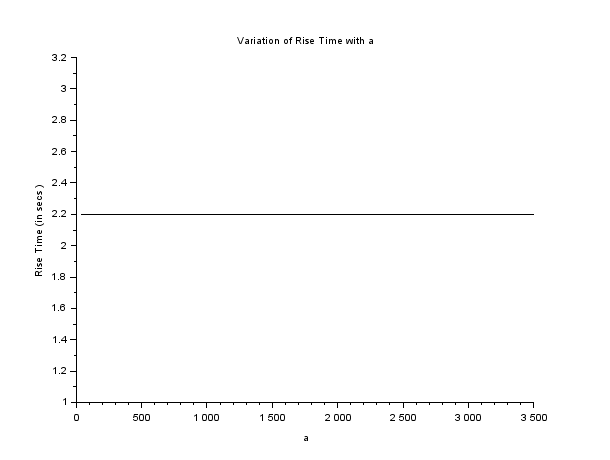
\includegraphics[scale=0.8]{q1_c.png}
        \caption{Rise Time vs 'a'}
        \label{fig:my_label}
    \end{figure}
  
\subsection*{Part d}  
    The rise time varies inversely with b, that is $RiseTime\propto\frac{1}{b}$, Its a rectangular hyperbola:-
    \begin{verbatim}
b = 1;
range_b = b:b:100*b;
range_rise_b = log(.9/.1)./range_b;
plot2d(range_b,range_rise_b);
xlabel ("b") ;
ylabel (" Rise Time (in secs )") ;
title (" Variation of Rise Time with b") ;
    \end{verbatim}
    \begin{figure}[H]
        \centering
        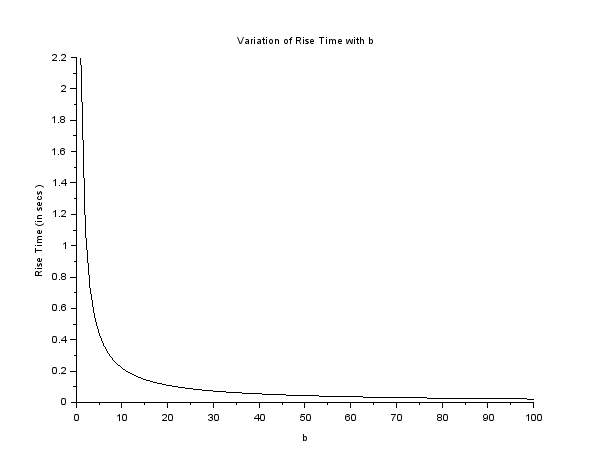
\includegraphics[scale=0.8]{q1_d.png}
        \caption{Rise Time vs 'b'}
        \label{fig:my_label}
    \end{figure}
    
\section{PROBLEM-2}
The entire code snippet :-
    \begin{figure}[H]
        \centering
        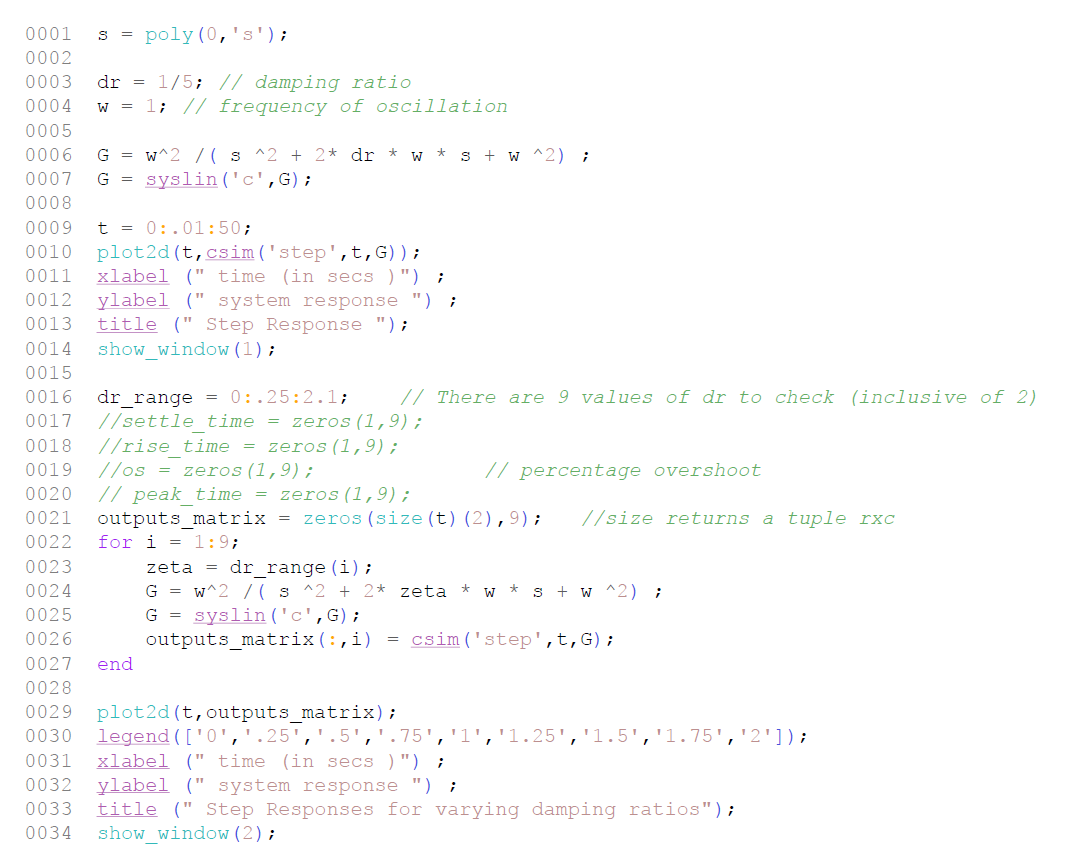
\includegraphics[scale=0.8]{q2_code.png}
    \end{figure}
\subsection*{Part a}  
    We know that such functions have the form:-
    \begin{align*}
        G = \frac{\omega_0^2}{s^2+2\zeta\omega_0s+\omega_0^2}
    \end{align*}
    Where $\zeta$ is the damping ratio, which needs to be between 0 and 1 for an underdamped system. 
\begin{itemize}
\item $\zeta$ = 1/5 for my system
\item w = 1 Hz since its standard
\end{itemize}
    \begin{verbatim}
s = poly(0,'s');
dr = 1/5; // damping ratio
w = 1; // frequency of oscillation

G = w^2 /( s ^2 + 2* dr * w * s + w ^2) ;
G = syslin('c',G);

t = 0:.01:50;
plot2d(t,csim('step',t,G));
xlabel (" time (in secs )") ;
ylabel (" system response ") ;
title (" Step Response ");
show_window(1);
    \end{verbatim}
    \begin{figure}[H]
        \centering
        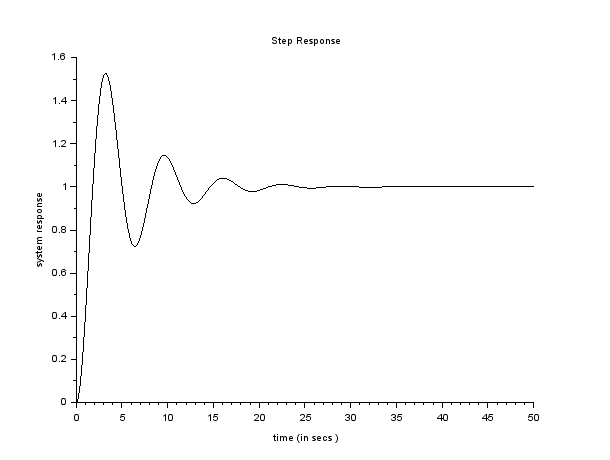
\includegraphics[scale=0.8]{q2_a}
        \caption{Step Response of Underdamped System with damping ratio=0.2}
        \label{fig:my_label}
    \end{figure}
 
\subsection*{Part b}     
 The step response of the systems with damping factor varying from 0.25 to 2 on the same plot are as follows:-
 The code for the above:-
    \begin{verbatim}
dr_range = 0:.25:2.1;    // There are 9 values of dr to check (inclusive of 2)
//settle_time = zeros(1,9);
//rise_time = zeros(1,9);
//os = zeros(1,9);              // percentage overshoot
// peak_time = zeros(1,9);
outputs_matrix = zeros(size(t)(2),9);   //size returns a tuple rxc
for i = 1:9;
    zeta = dr_range(i);
    G = w^2 /( s ^2 + 2* zeta * w * s + w ^2) ;
    G = syslin('c',G);
    outputs_matrix(:,i) = csim('step',t,G);
end

plot2d(t,outputs_matrix);
legend(['0','.25','.5','.75','1','1.25','1.5','1.75','2']);
xlabel (" time (in secs )") ;
ylabel (" system response ") ;
title (" Step Responses for varying damping ratios");
show_window(2);
    \end{verbatim}
    \begin{figure}[H]
        \centering
        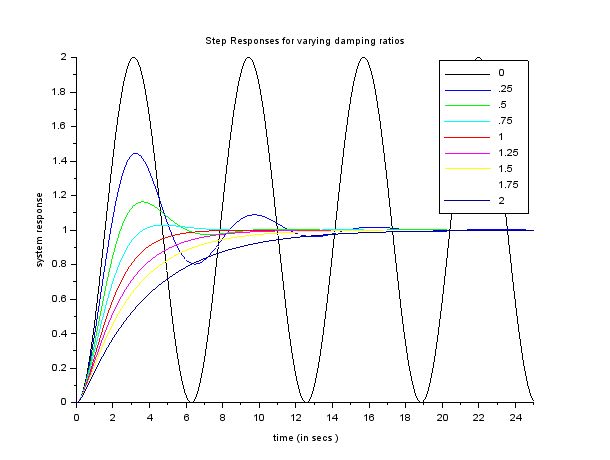
\includegraphics[scale=0.8]{q2_b.png}
        \caption{Varying Damping Ratio from 0 to 2}
        \label{fig:my_label}
    \end{figure}  
\begin{itemize}
\item Rise time and peak time remain approximately same for increasing damping ratio
\item Overshoot percentage decreases with increasing zeta
\item 2\% settle time decreases with increasing zeta in underdamped regime
\end{itemize}
%    Now, the plots comparing percentage overshoot, rise time, 2\% settling time and peak-time change are as follows:-
%    \begin{figure}[H]
%        \begin{subfigure}{.5\textwidth}
%            \centering
%            \includegraphics[width=.8\linewidth]{2-4.jpg}  
%            \caption{Rise Time vs Damping Factor}
%            \label{fig:sub-first}
%        \end{subfigure}
%        \hfill
%        \begin{subfigure}{.5\textwidth}
%            \centering
%            \includegraphics[width=.8\linewidth]{2-5.jpg}  
%            \caption{Overshoot vs Damping Factor}
%            \label{fig:sub-second}
%        \end{subfigure}
%        \newline
%        \begin{subfigure}{.5\textwidth}
%            \centering
%            \includegraphics[width=.8\linewidth]{2-6.jpg}  
%            \caption{Settling Time vs Damping Factor}
%            \label{fig:sub-first}
%        \end{subfigure}
%        \hfill
%        \begin{subfigure}{.5\textwidth}
%            \centering
%            \includegraphics[width=.8\linewidth]{2-7.jpg}  
%            \caption{Peak Time vs Damping Factor}
%            \label{fig:sub-second}
%        \end{subfigure}
%        \caption{Variation of various quantities with damping factor}
%        \label{fig:fig}
%    \end{figure}
%    The code for implementing the following were:-
%    \begin{verbatim}
%    S = stepinfo(H);
%    figure
%    plot(zeta, [S.RiseTime])
%    figure
%    plot(zeta, [S.Overshoot])
%    figure
%    plot(zeta, [S.SettlingTime])
%    figure
%    plot(zeta, [S.PeakTime])
%    \end{verbatim}

\section{PROBLEM-3}
The entire code snippet :-
    \begin{figure}[H]
        \centering
        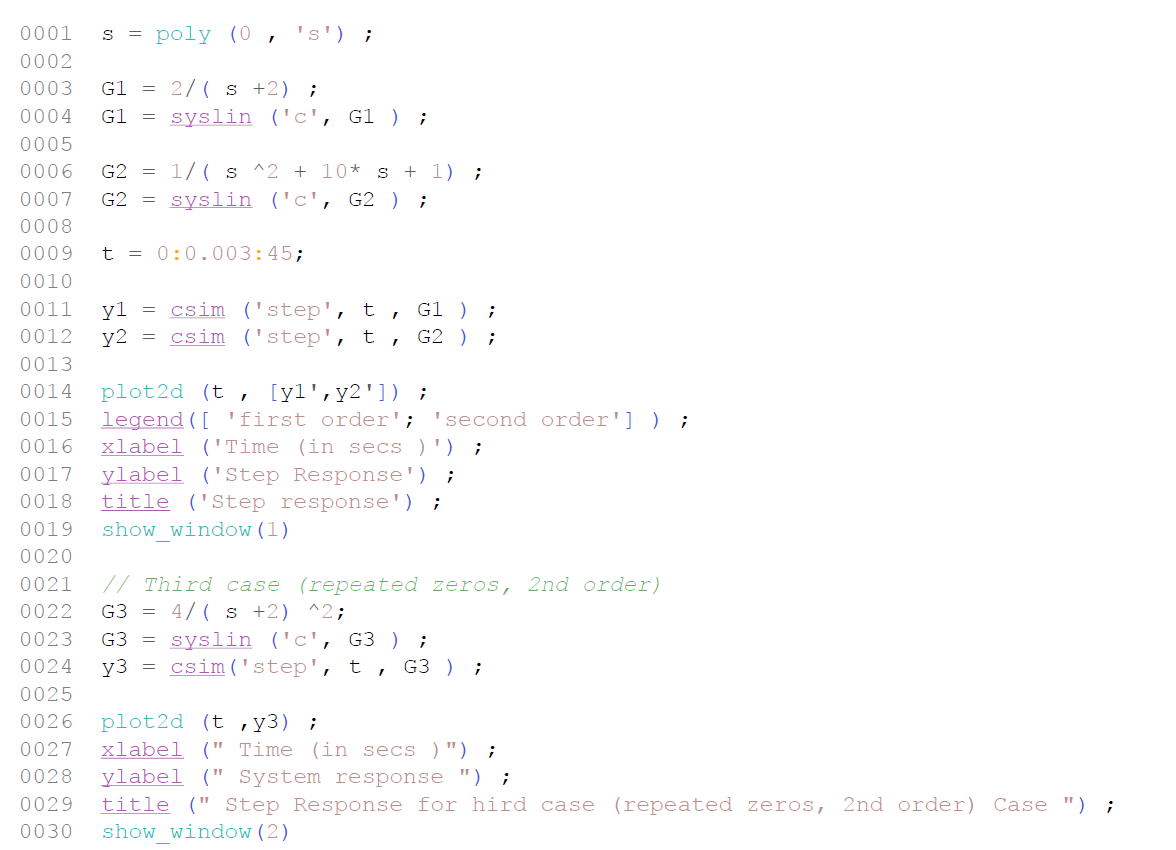
\includegraphics[scale=0.8]{q3_code.png}
    \end{figure}
    The chosen first order and second order system are:-
    \begin{align*}
        & G_1(s) = \frac{2}{s+2} \\
        & G_2(s) = \frac{1}{s^2+10s+1}
    \end{align*}
The code for this part is:-
    \begin{verbatim}
s = poly (0 , 's') ;

G1 = 2/( s +2) ;
G1 = syslin ('c', G1 ) ;

G2 = 1/( s ^2 + 10* s + 1) ;
G2 = syslin ('c', G2 ) ;

t = 0:0.003:45;


y1 = csim ('step', t , G1 ) ;
y2 = csim ('step', t , G2 ) ;

plot2d (t , [y1',y2']) ;
legend([ 'first order'; 'second order'] ) ;
xlabel ('Time (in secs )') ;
ylabel ('Step Response') ;
title ('Step response') ;
show_window(1)
    \end{verbatim}

    The step response obtained is:-
    \begin{figure}[H]
        \centering
        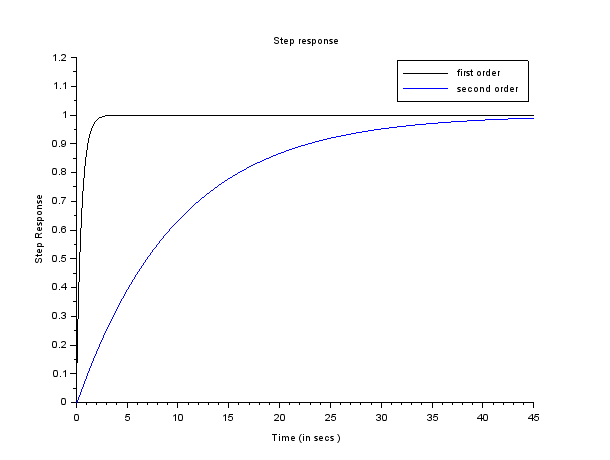
\includegraphics[scale=0.8]{q3_1.png}
        \caption{First Order vs Second Order step response}
        \label{fig:my_label}
    \end{figure}
    The differences between the two were:-
    \begin{itemize}
        \item The first order response had a smaller Rise Time \vspace{-2.5pt}
        \item The first order response had a smaller Settling Time
	\item The first order response approaches the equilibrium more quickly than the second order response.
\item Derivative is 0 for 2nd order response at t =0 wherease first order has a non-zero derivative
    \end{itemize}

    In case of repeated roots, transfer function was:-
    \begin{align*}
        G_3(s) = \frac{4}{s^2+4s+4}
    \end{align*}
    The step response was indeed monotonic as can be seen below:-
    \begin{figure}[H]
        \centering
        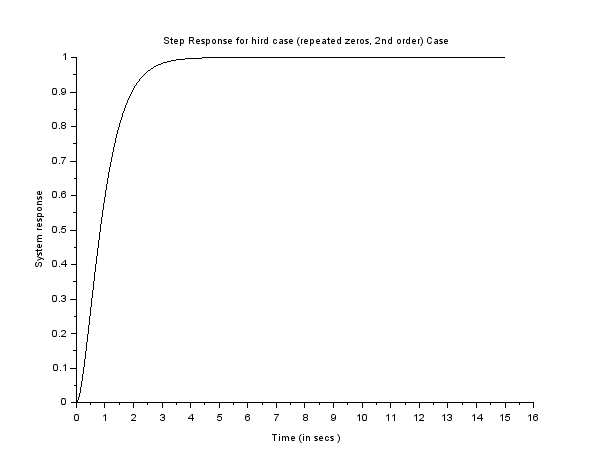
\includegraphics[scale=0.8]{q3_2.png}
        \caption{Repeated Pole Second Order Step Response}
        \label{fig:my_label}
    \end{figure}

    The code for this question was as follows:-
    \begin{verbatim}
G3 = 4/( s +2) ^2;
G3 = syslin ('c', G3 ) ;
y3 = csim('step', t , G3 ) ;

plot2d (t ,y3) ;
xlabel (" Time (in secs )") ;
ylabel (" System response ") ;
title (" Step Response for hird case (repeated zeros, 2nd order) Case ") ;
show_window(2)
    \end{verbatim}
    
\section{PROBLEM-4}
The entire code snippet :-
    \begin{figure}[H]
        \centering
        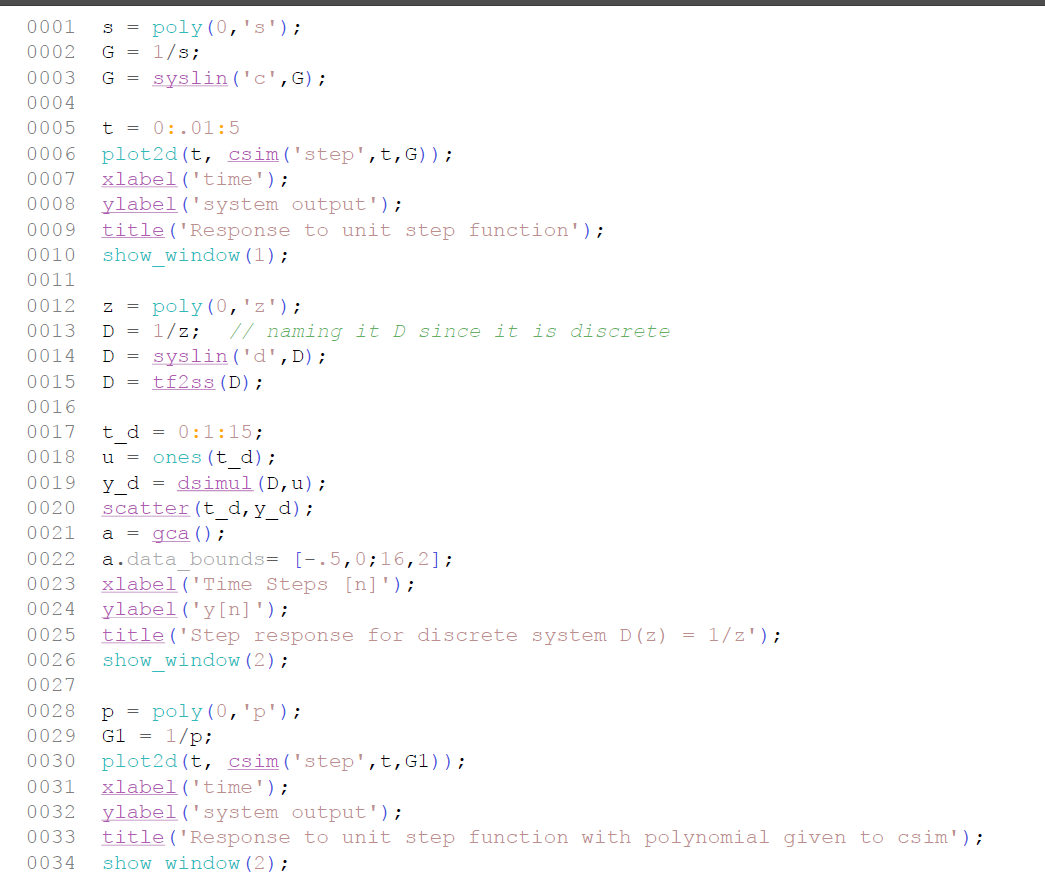
\includegraphics[scale=0.8]{q4_code.png}
    \end{figure}
The code for a part is :-
\begin{verbatim}
s = poly(0,'s');
G = 1/s;
G = syslin('c',G);

t = 0:.01:5
plot2d(t, csim('step',t,G));
xlabel('time');
ylabel('system output');
title('Response to unit step function');
show_window(1);
    \end{verbatim}
 The step response obtained is:-
    \begin{figure}[H]
        \centering
        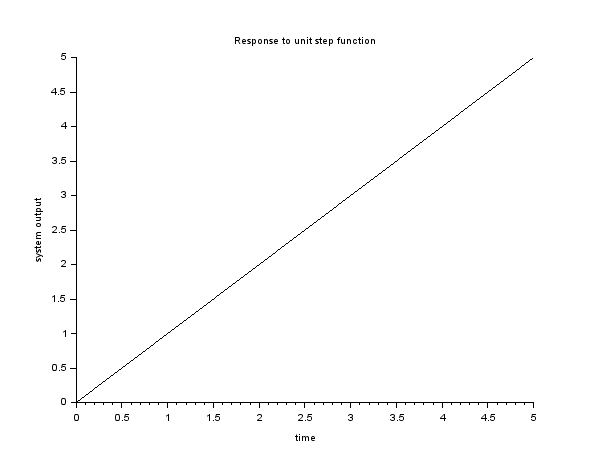
\includegraphics[scale=0.8]{q4_a.png}
        \caption{Continuous step response for 1/s}
        \label{fig:my_label}
    \end{figure}
\textbf{We see that while in continuous time, a transfer function of the form $\frac{1}{s}$ acts as an integrator}

The code for b part is :-
\begin{verbatim}
z = poly(0,'z');
D = 1/z;  // naming it D since it is discrete
D = syslin('d',D);
D = tf2ss(D);

t_d = 0:1:15;
u = ones(t_d);
y_d = dsimul(D,u);
scatter(t_d,y_d);
a = gca();
a.data_bounds= [-.5,0;16,2];
xlabel('Time Steps [n]');
ylabel('y[n]');
title('Step response for discrete system D(z) = 1/z');
show_window(2);
    \end{verbatim}   
 The step response obtained is:-
    \begin{figure}[H]
        \centering
        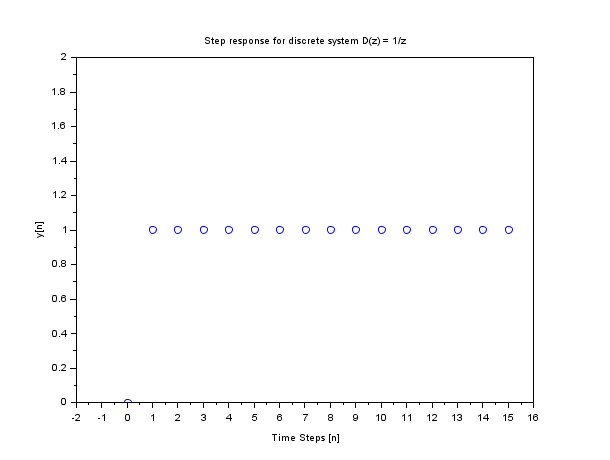
\includegraphics[scale=0.8]{q4_b.png}
        \caption{Discrete time step response for 1/z}
        \label{fig:my_label}
    \end{figure}
\textbf{in discrete time, the transfer function $\frac{1}{z}$ acts as a time delayer since in the Z-domain, a multiplication with $\frac{1}{z}$ indicates a time delay of 1 unit}

The code for c part is :-
\begin{verbatim}
p = poly(0,'p');
G1 = 1/p;
plot2d(t, csim('step',t,G1));
xlabel('time');
ylabel('system output');
title('Response to unit step function with polynomial given to csim');
show_window(2);
    \end{verbatim}   
 The step response obtained is:-
    \begin{figure}[H]
        \centering
        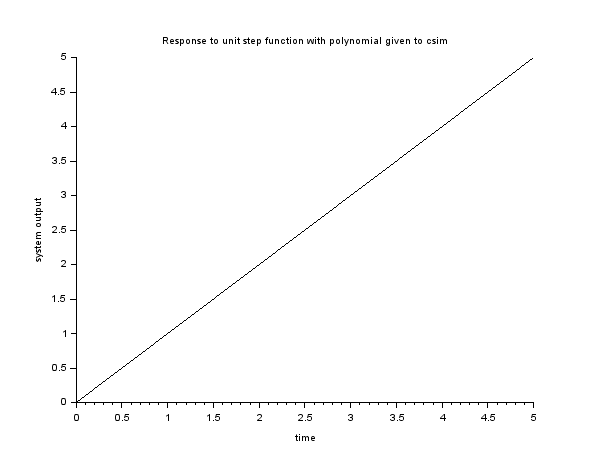
\includegraphics[scale=0.8]{q4_c.png}
        \caption{step response for polynomial 1/p}
        \label{fig:my_label}
    \end{figure}

\textbf{I personally didn't get any error after passing a polynomial to csim function however got a warning --- WARNING: csim: Input argument \#1 is assumed continuous time.}

\section{PROBLEM-5}
The entire code snippet :-
    \begin{figure}[H]
        \centering
        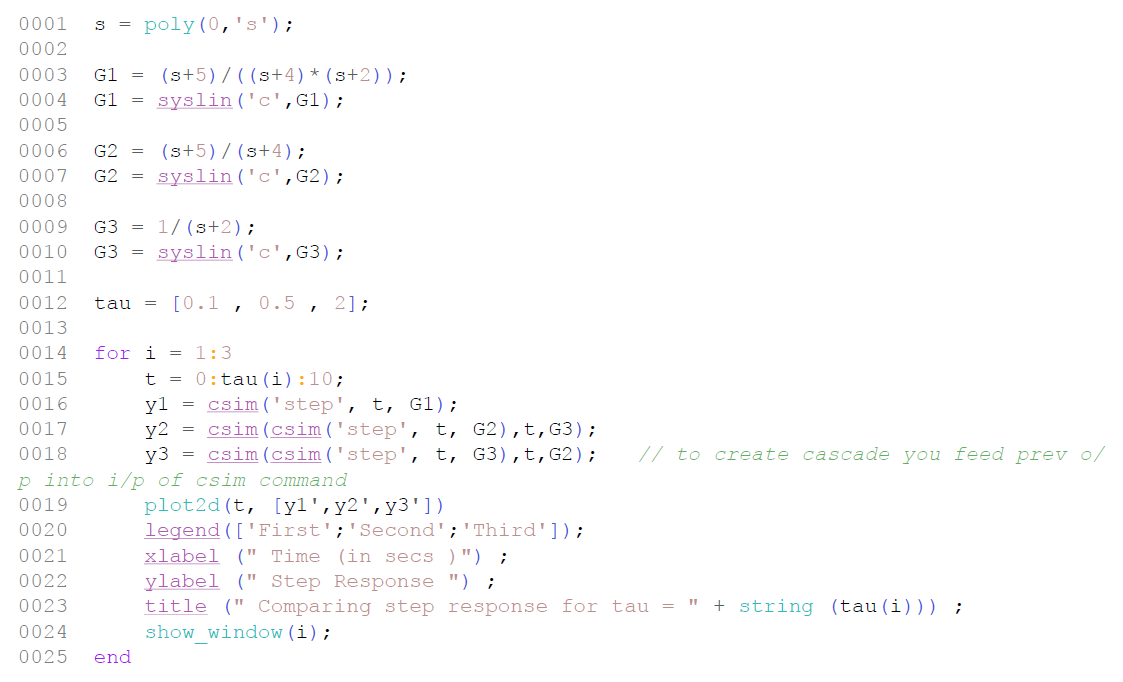
\includegraphics[scale=0.8]{q5_code.png}
    \end{figure}
    On plotting, we observe the following 3 plots:-
    
    \begin{figure}[H]
        \begin{subfigure}{.5\textwidth}
            \centering
            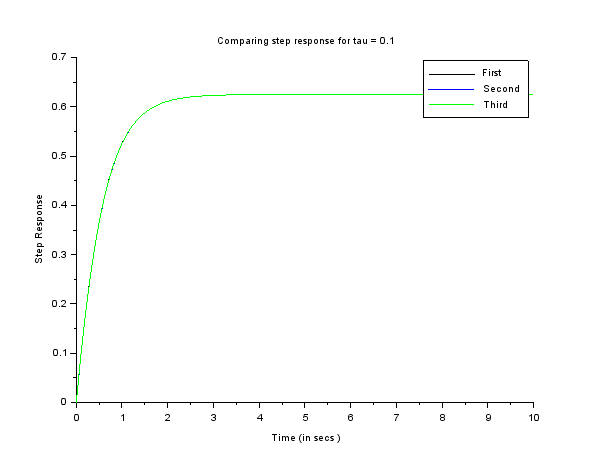
\includegraphics[width=.8\linewidth]{q5_1st_value.png}  
            \caption{$\tau$=0.1s}
            \label{fig:sub-first}
        \end{subfigure}
        \hfill
        \begin{subfigure}{.5\textwidth}
            \centering
            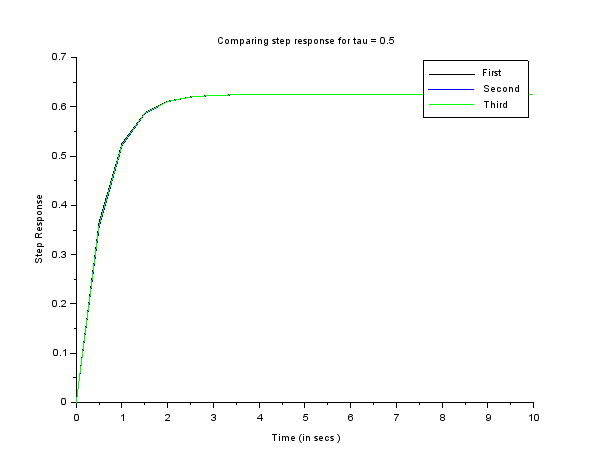
\includegraphics[width=.8\linewidth]{q5_2nd_value.png}  
            \caption{$\tau$=0.2s}
            \label{fig:sub-second}
        \end{subfigure}
        \newline
        \begin{subfigure}{\textwidth}
            \centering
            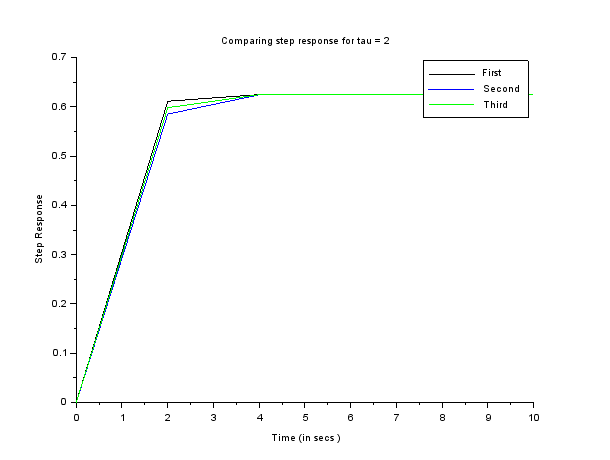
\includegraphics[width=.8\linewidth]{q5_2.png}  
            \caption{$\tau$=2s}
            \label{fig:sub-first}
        \end{subfigure}
        \caption{The Three output graphs with varying sampling period($\tau$)}
        \label{fig:fig}
    \end{figure}
    As one can clearly see, no observable error pops up when $\tau=0.1s$ and when $\tau=0.2s$. However, an error does appear when we change to $\tau=2s$.
\end{document}
